% Architecture review for the multi-agent paradigm-shift simulation.
% Compile:  pdflatex architecture_review.tex
% Companion to notes/theory_brief.md (2026-05-08).

\documentclass[11pt,a4paper]{article}

\usepackage[margin=1in]{geometry}
\usepackage{amsmath,amssymb}
\usepackage{booktabs}
\usepackage{microtype}
\usepackage{xcolor}
\usepackage{enumitem}
\usepackage{hyperref}
\usepackage{tikz}
\usetikzlibrary{arrows.meta,positioning,fit,backgrounds,calc,shapes.geometric}

\hypersetup{colorlinks=true, linkcolor=blue!50!black,
            citecolor=blue!50!black, urlcolor=blue!50!black}

% Colour palette for diagrams ------------------------------------------------
\definecolor{flagred}{RGB}{200,40,40}
\definecolor{okgreen}{RGB}{40,140,60}
\definecolor{boxblue}{RGB}{40,90,160}
\definecolor{boxgrey}{RGB}{120,120,120}
\definecolor{boxorange}{RGB}{210,120,30}

\tikzset{
  proc/.style    = {rectangle, rounded corners=2pt, draw=boxblue, fill=boxblue!8,
                    thick, minimum height=9mm, minimum width=26mm,
                    align=center, font=\small},
  procfix/.style = {rectangle, rounded corners=2pt, draw=okgreen!70!black,
                    fill=okgreen!10, thick, minimum height=9mm, minimum width=26mm,
                    align=center, font=\small},
  state/.style   = {rectangle, rounded corners=2pt, draw=boxgrey, fill=boxgrey!8,
                    thick, minimum height=9mm, minimum width=24mm,
                    align=center, font=\small},
  env/.style     = {ellipse, draw=boxorange!80!black, fill=boxorange!12, thick,
                    minimum height=9mm, minimum width=26mm, align=center, font=\small},
  flag/.style    = {rectangle, rounded corners=2pt, draw=flagred, fill=flagred!10,
                    thick, align=center, font=\footnotesize\itshape, text=flagred,
                    inner sep=3pt},
  arr/.style     = {-{Stealth[length=2.5mm]}, thick, draw=boxblue!80},
  arrloop/.style = {-{Stealth[length=2.5mm]}, thick, draw=boxgrey!80, dashed},
}

\newcommand{\code}[1]{\texttt{\small #1}}

% --------------------------------------------------------------------------
\title{Architecture review: from single-shot Eq.\,13 \\
       to a recursive active-inference filter}
\author{Paradigm-Shift Active Inference --- IWAI 2026 \\
        \small companion to \texttt{notes/theory\_brief.md}}
\date{2026-05-09}

\begin{document}
\maketitle

\begin{abstract}
\noindent The v02 implementation applies Hyland \& Albarracin (2025)'s
closed-form $\lambda$-conservatism update (Eq.~13) recursively as a sequential
filter. This produces unbounded log-posterior accumulation: under steady
evidence, $|C_t|$ grows linearly in $t$ until saturation pins every agent into
total commitment. A memory-decay patch ($\beta = 0.95$ on $C_{\text{old}}$)
bounded the magnitude empirically but smuggled a transition model into the
wrong place. This note diagnoses four design shortcuts behind the pathology,
reads them through the lenses of three reviewers (Hyland on active inference,
Leibo on multi-agent norm dynamics, Tan Zhi-Xuan on Bayesian theory of mind),
and lays out a four-piece fix that re-grounds the simulation in proper
recursive active inference. Two TikZ flowcharts contrast the current and
proposed information loops.
\end{abstract}

% --------------------------------------------------------------------------
\section{Where we started}
\label{sec:plan}

The theory brief (\code{notes/theory\_brief.md}, 2026-05-08) specified a
$N=30$ agent model on a Watts--Strogatz small-world graph. Each agent
$i$ carries log-preferences $C_i \in \mathbb{R}^{|\mathcal{O}|}$, edge
precisions $\{\gamma_{ij}\}$, delegation $d_i \in [0,1]$ and
cost-of-mind-change $\lambda_i \geq 0$. Two evidence streams (environmental,
social) are aggregated into a per-step posterior; the headline empirical
target is a $(\lambda, \text{drift rate})$ phase diagram with hysteresis.

The brief offered two candidate $C$-update forms:
\begin{align}
\textbf{(a) gradient on KL+}\lambda\textbf{KL:} \quad
   C_i^{(t+1)} &= \arg\min_C \Bigl[\,
      \mathrm{KL}\bigl[q_i^{(t+1)} \,\|\, p(o\mid C)\bigr]
      + \lambda_i \,\mathrm{KL}\bigl[p(o\mid C) \,\|\, p(o\mid C_i^{(t)})\bigr]
   \Bigr], \label{eq:gd-form}\\[2pt]
\textbf{(b) closed-form Eq.\,13:} \quad
   q^*(s) &\propto p(s) \cdot \exp\!\bigl[\lambda^{-1} \cdot (-F(s))\bigr]. \label{eq:eq13}
\end{align}
\eqref{eq:gd-form} requires an inner gradient loop per agent per step;
\eqref{eq:eq13} is closed-form. We chose (b) for v02 of the implementation
because it is fast and is the form Hyland publishes.

% --------------------------------------------------------------------------
\section{Where we got to}
\label{sec:impl}

The current code path lives in \code{src/population.py::\_observe\_jit}
(lines 138--180). At each step:
\begin{enumerate}[topsep=2pt,itemsep=2pt]
\item \textbf{Env channel.} \code{pymdp.infer\_states(obs, empirical\_prior=D)}
  returns a per-agent posterior $p_{\text{env}}$.
\item \textbf{Social channel.} A trust-weighted pool over neighbours' previous
  posteriors gives $p_{\text{social}}$.
\item \textbf{Belief update.} The pseudo-recursive form
  \begin{equation}
  C_t \;=\; \beta\,C_{t-1} \;+\; \lambda^{-1}\bigl[\, d\,\log p_{\text{social}}
                                             + (1-d)\,\log p_{\text{env}} \bigr],
  \label{eq:current-update}
  \end{equation}
  with $\beta = 0.95$ added in the most recent slice to bound $|C_t|$.
\item \textbf{Action.} $a_i \sim \mathrm{softmax}(C_t)$.
\item \textbf{Trust update.} $\gamma_{ij} \mathrel{*}= \exp(-\eta \cdot \mathrm{NLL}_j)$.
\end{enumerate}

The pymdp generative model is intentionally trivial: $A = I_{n_o}$,
$B = I_{n_o}$ (single null control), $D$ uniform.

\paragraph{What works.} Heterogeneous-$\lambda$ slow-drift rollouts produce a
visible cascade signature: low-$\lambda$ agents sign-flip first, drag
neighbours along on a delay (\code{notebooks/02\_phase\_space.ipynb}, \S4).

\paragraph{What doesn't.}
\begin{enumerate}[topsep=2pt,itemsep=2pt]
\item Without $\beta$, $|C_t|$ runs to $\pm 10^4$ within $\sim$300 steps under
  consistent evidence. Posterior is then $\sim$one-hot regardless of
  subsequent observations: agents cannot recover from the wrong belief.
\item With $\beta = 0.95$, the equilibrium $|C_\infty| = e/(\lambda(1-\beta))$
  saturates in $\sim$20 steps regardless of $\lambda$. The phase grid is
  $\lambda$-flat at the resolution we measured.
\item The $\lambda$-cascade in (\S4 of the notebook) is real but lives in
  a narrow window before saturation.
\end{enumerate}

% --------------------------------------------------------------------------
\section{Diagnosis: four shortcuts}
\label{sec:diag}

Figure~\ref{fig:current} traces the information loops in the current
implementation. Two pieces are flagged on the diagram itself; two more are
algebraic, given below the figure.

\begin{figure}[ht]
\centering
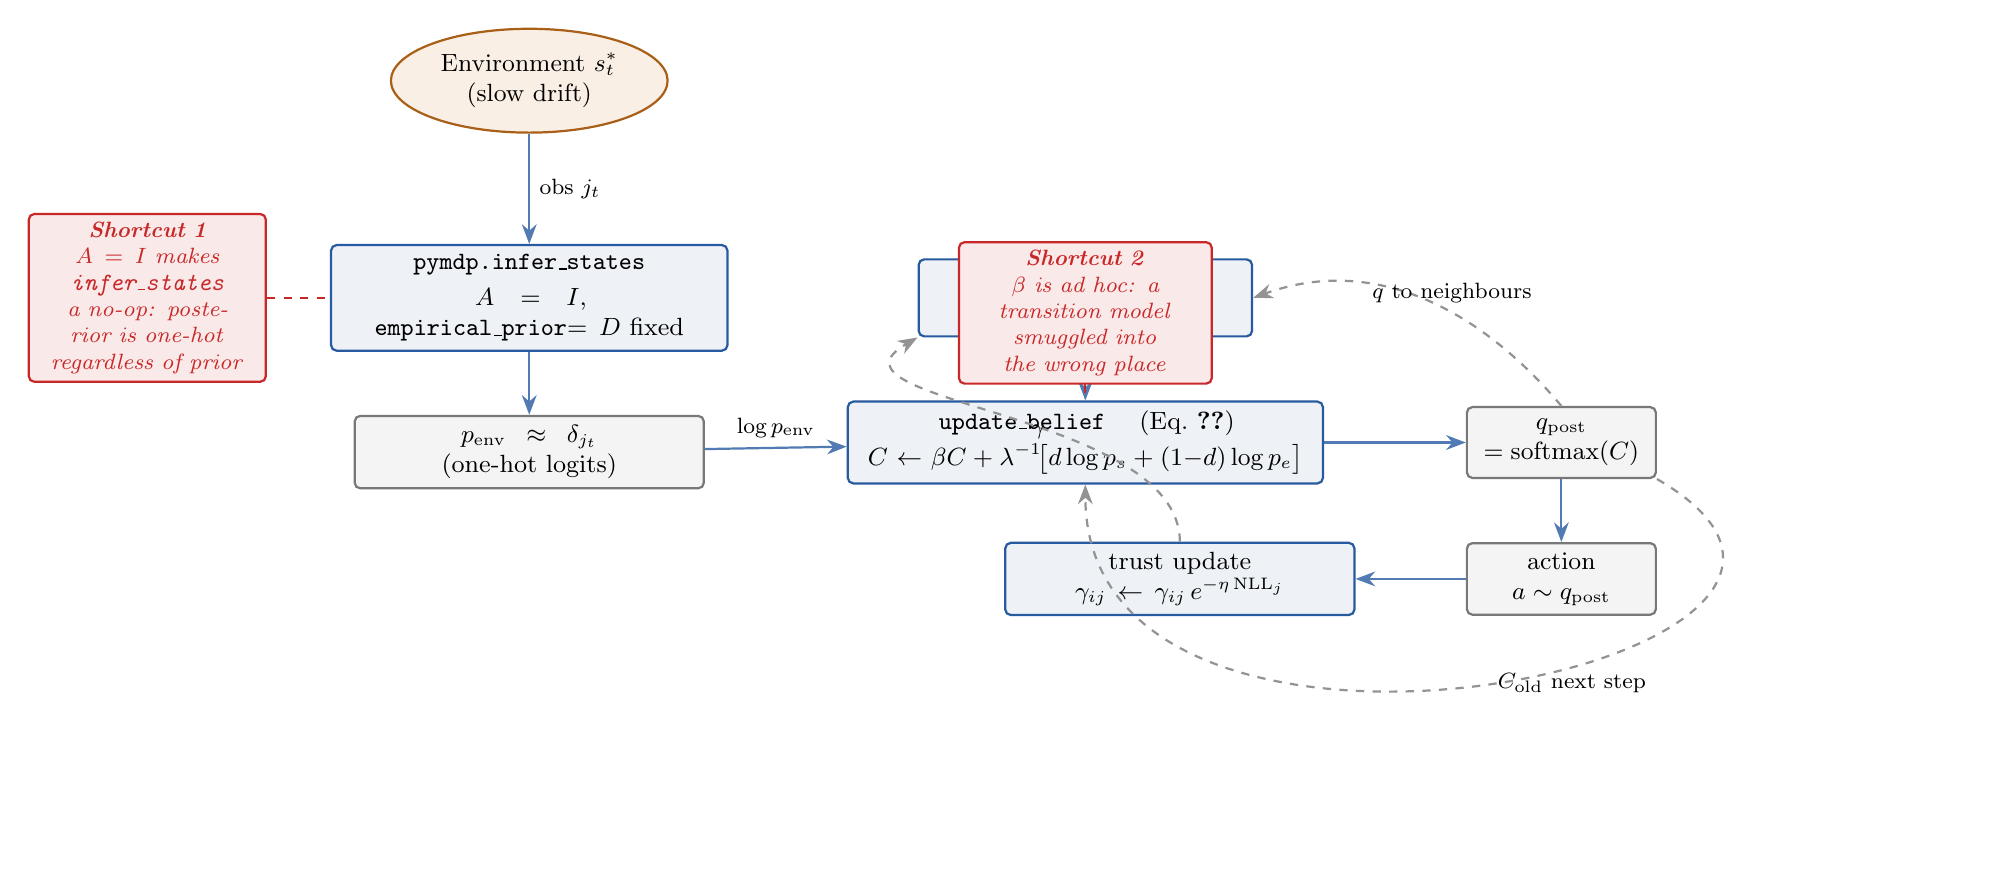
\begin{tikzpicture}[node distance=10mm and 18mm]

% Environment
\node[env] (env) {Environment $s^*_t$\\(slow drift)};

% pymdp inference
\node[proc, below=14mm of env, text width=48mm] (infer) {%
  \code{pymdp.infer\_states}\\[2pt]
  $A = I$,\; \code{empirical\_prior}$=D$ fixed
};
\draw[arr] (env) -- node[right, font=\footnotesize] {obs $j_t$} (infer);

% p_env state
\node[state, below=8mm of infer, text width=42mm] (penv) {$p_{\text{env}} \approx \delta_{j_t}$\\(one-hot logits)};
\draw[arr] (infer) -- (penv);

% neighbour pool above-right of update
\node[proc, right=24mm of infer, text width=40mm] (npool) {%
  neighbour pool\\$p_{\text{social}} = \sum_j \gamma_{ij}\,q_j$
};

% update_belief
\node[proc, below=8mm of npool, text width=58mm] (upd) {%
  \code{update\_belief} \quad (Eq.~\ref{eq:current-update})\\[2pt]
  $C \leftarrow \beta C + \lambda^{-1}\!\bigl[d\log p_s + (1{-}d)\log p_e\bigr]$
};
\draw[arr] (npool) -- node[right, font=\footnotesize] {$p_{\text{social}}$} (upd);
\draw[arr] (penv) -- node[above, font=\footnotesize] {$\log p_{\text{env}}$} (upd);

% q_post
\node[state, right=18mm of upd] (qpost) {$q_{\text{post}}$\\$=\mathrm{softmax}(C)$};
\draw[arr] (upd) -- (qpost);

% action
\node[state, below=8mm of qpost] (act) {action\\$a \sim q_{\text{post}}$};
\draw[arr] (qpost) -- (act);

% trust update
\node[proc, left=14mm of act, text width=42mm] (trust) {trust update\\$\gamma_{ij}\!\leftarrow\!\gamma_{ij}\,e^{-\eta\,\mathrm{NLL}_j}$};
\draw[arr] (act) -- (trust);

% temporal feedback q_post -> next step's C_old
\draw[arrloop] (qpost.south east) to[out=-30, in=-90, looseness=1.6]
   node[right, font=\footnotesize, pos=0.5] {$C_{\text{old}}$ next step}
   (upd.south);

% q_post -> neighbour_pool (other agents)
\draw[arrloop] (qpost.north) to[out=130, in=20]
   node[above, font=\footnotesize, pos=0.4] {$q$ to neighbours}
   (npool.east);

% trust feeds neighbour_pool
\draw[arrloop] (trust.north) to[out=90, in=-150]
   node[left, font=\footnotesize, pos=0.4] {$\gamma$}
   (npool.south west);

% Flags ----------------------------------------------------------------
\node[flag, left=8mm of infer.west, text width=28mm] (f1)
   {\textbf{Shortcut 1}\\$A=I$ makes \code{infer\_states} a no-op:
    posterior is one-hot regardless of prior};
\draw[draw=flagred, dashed, thick] (f1.east) -- (infer.west);

\node[flag, above=2mm of upd.north, text width=30mm] (f2)
   {\textbf{Shortcut 2}\\$\beta$ is ad hoc: a transition model
    smuggled into the wrong place};
\draw[draw=flagred, dashed, thick] (f2.south) -- (upd.north);

\end{tikzpicture}
\caption{Information flow in the v02 implementation. Solid arrows are
within-step computation; dashed arrows are state that feeds back into the
next step. Two of the four diagnosed shortcuts are algebraic and shown
inline below the figure.}
\label{fig:current}
\end{figure}

\paragraph{Shortcut 1: $A = I$ makes \code{infer\_states} a no-op.}
With identity observation likelihood, posterior $\propto A[\text{obs},\,:]\cdot
\text{prior} = e_{\text{obs}}\cdot\text{prior}$, which after normalisation is
$\delta_{\text{obs}}$ regardless of the prior. So whatever we feed as
\code{empirical\_prior} is overwhelmed by the observation. The pymdp
machinery is paying compilation cost for what is mathematically a dictionary
lookup.

\paragraph{Shortcut 2: the $\beta$ patch.}
\eqref{eq:current-update} with $\beta < 1$ is a linear filter on $C$ with
geometric memory. It bounds $|C_t|$ at $e/(\lambda(1-\beta))$ under steady
evidence $e$, but the time constant $1/(1-\beta)$ is independent of $\lambda$.
$\lambda$ now controls the magnitude of equilibrium confidence, not the speed
of belief change. That is not what $\lambda$ is supposed to do in
\eqref{eq:eq13}.

\paragraph{Shortcut 3: \eqref{eq:eq13} is single-shot.}
Hyland \& Albarracin's Eq.~13 is a variational solution at one inference step,
with $p(s)$ the generative model's prior --- fixed. Our recursion
$p_t = q_{t-1}$ (i.e.\ yesterday's posterior is today's prior) is not in the
paper. With no transition model in $B$, log-posterior magnitude grows
linearly in $t$ forever. This is the actual root cause of the runaway; the
$\beta$ patch hides it without addressing it.

\paragraph{Shortcut 4: the social channel is a flat opinion pool.}
$p_{\text{social}} = \sum_j \gamma_{ij}\,q_j$ has no structure: agents do
not represent why a neighbour holds their belief. The mixing of
$\log p_{\text{env}}$ and $\log p_{\text{social}}$ via $d$ is also an
extension to \eqref{eq:eq13} that needs justification or it becomes a free
parameter that does whatever we want.

% --------------------------------------------------------------------------
\section{Three perspectives}
\label{sec:perspectives}

The four shortcuts are not equally severe under different lenses.

\paragraph{Hyland (active inference orthodoxy).} Shortcuts 1 and 3 are the
load-bearing problems. \code{pymdp.Agent} already exposes $A$ and $B$;
softening both would let pymdp's variational machinery do real recursive
filtering, and the $\beta$ patch becomes unnecessary. Hyland would also
question the $d$-weighted log-mixing in shortcut 4: there is a coherent
two-likelihood form (Section~\ref{sec:fix}) that respects the variational
geometry.

\paragraph{Leibo (multi-agent / norm dynamics).} The pathology Leibo would
flag first is independent of the four shortcuts: \emph{agents observe each
other's posteriors, not their actions} (\code{population.py:158}, where
\code{pop.q\_post} flows directly into \code{neighbour\_pool}). In real norm
learning, behaviour is observed, not belief: actions are downstream of belief
$\times$ utility $\times$ noise, and that noise is what regularises social
inference. Removing the action channel removes the regularisation. Compounding
this, the trust update reinforces homophily without an exploration
counter-pressure: agreement on wrong answers keeps $\gamma$ high; the model
has no parameter regime that produces a paradigm shift instead of lock-in,
which a model of paradigm shifts ought to.

\paragraph{Tan Zhi-Xuan (Bayesian ToM).} Each agent should maintain a
posterior over each neighbour's belief and reliability, not just a scalar
trust. The current $\gamma_{ij}$ is a heuristic decay on outcome agreement;
ZX's frame would have $\gamma_{ij}$ derived from predictive-accuracy Bayes,
with separate uncertainty about the neighbour's $\lambda$ (deliberate vs.
impulsive). This is a substantial structural addition and is out of scope for
the current slice.

% --------------------------------------------------------------------------
\section{Proposed fix}
\label{sec:fix}

The agreed direction (\textbf{Replace} $\beta$ \textbf{with B-matrix drift})
turns out to require four coordinated changes once we look at the actual A/B
construction. Each piece is paper-defensible on its own, and together they
restore proper recursive active inference.

\begin{table}[h]
\centering
\small
\begin{tabular}{@{}l p{55mm} p{55mm}@{}}
\toprule
\textbf{Piece} & \textbf{Current} & \textbf{Proposed} \\
\midrule
$A$ & $I_{n_o}$ & $(1-\nu)\,I + \nu\,(\mathbf{1}\mathbf{1}^\top - I)/(n_o{-}1)$ \\
$B$ & $I_{n_o}$ & $(1-\varepsilon)\,I + \varepsilon\,\mathbf{1}\mathbf{1}^\top/n_o$ \\
\code{empirical\_prior} & $D$ (fixed uniform) & $q_{\text{post},\,t-1}$ (recursive) \\
update rule & $C_t = \beta\,C_{t-1} + \lambda^{-1}\!\log\text{evidence}$ &
   $q_t \propto (B\,q_{t-1}) \cdot p_{\text{env}}^{(1-d)/\lambda}\cdot
                 p_{\text{social}}^{d/\lambda}$ \\
\bottomrule
\end{tabular}
\caption{Four-piece architectural change. New parameters: observation noise
$\nu$ (default $0.05$), state-drift $\varepsilon$ (default $0.02$). The
$\beta$ memory parameter is removed.}
\label{tab:fix}
\end{table}

\paragraph{Why this works.} Under steady evidence $e$, the proposed
update has $q_t \propto B\,q_{t-1} \cdot p_{\text{env}}^{1/\lambda}$. The
factor $B\,q_{t-1}$ is bounded below by $\varepsilon/n_o$ in every component,
so $\log q_t$ is bounded above. $\lambda$ now controls the \emph{strength} of
the likelihood relative to the prior at every step --- exactly the role
Eq.~\ref{eq:eq13} gives it --- without needing memory decay to keep things
finite. The temporal coupling lives in $B$, where active-inference theory
expects it.

\paragraph{Equilibrium analysis (sketch).} Fix $d=0$ (env channel only),
steady observation $j$, scalar $\lambda$. The fixed-point posterior $q^*$
satisfies
\[
q^*(s) \;\propto\; \bigl[(1-\varepsilon)q^*(s) + \varepsilon/n_o\bigr]
                   \cdot p(o = j \mid s)^{1/\lambda},
\]
which has a unique attractor with $q^*(j) < 1$ when $\varepsilon > 0$. As
$\varepsilon \to 0$ recovery is impossible (the current pathology); as
$\varepsilon \to 1$ no learning occurs (uninformative prior every step).
$\lambda$ shifts the location of the attractor smoothly: low $\lambda$
$\Rightarrow$ sharper $q^*$, high $\lambda$ $\Rightarrow$ flatter $q^*$.
That is what the brief's Predicted Phenomena table assumes.

\paragraph{The social-channel choice.} The proposed update treats
$p_{\text{env}}$ and $p_{\text{social}}$ as two independent likelihoods, each
tempered by its own weight on $1/\lambda$. This is mathematically clean
($q_t$ is still proportional to a product of distributions) and reduces to
\eqref{eq:eq13} when $d = 0$. It changes one thing relative to the current
mix: under low $\lambda$, the social channel gets sharpened the same way the
env channel does, so cascade signatures should be cleaner, not noisier. We
adopt this form.

\medskip
Figure~\ref{fig:proposed} shows the resulting information flow.

\begin{figure}[ht]
\centering
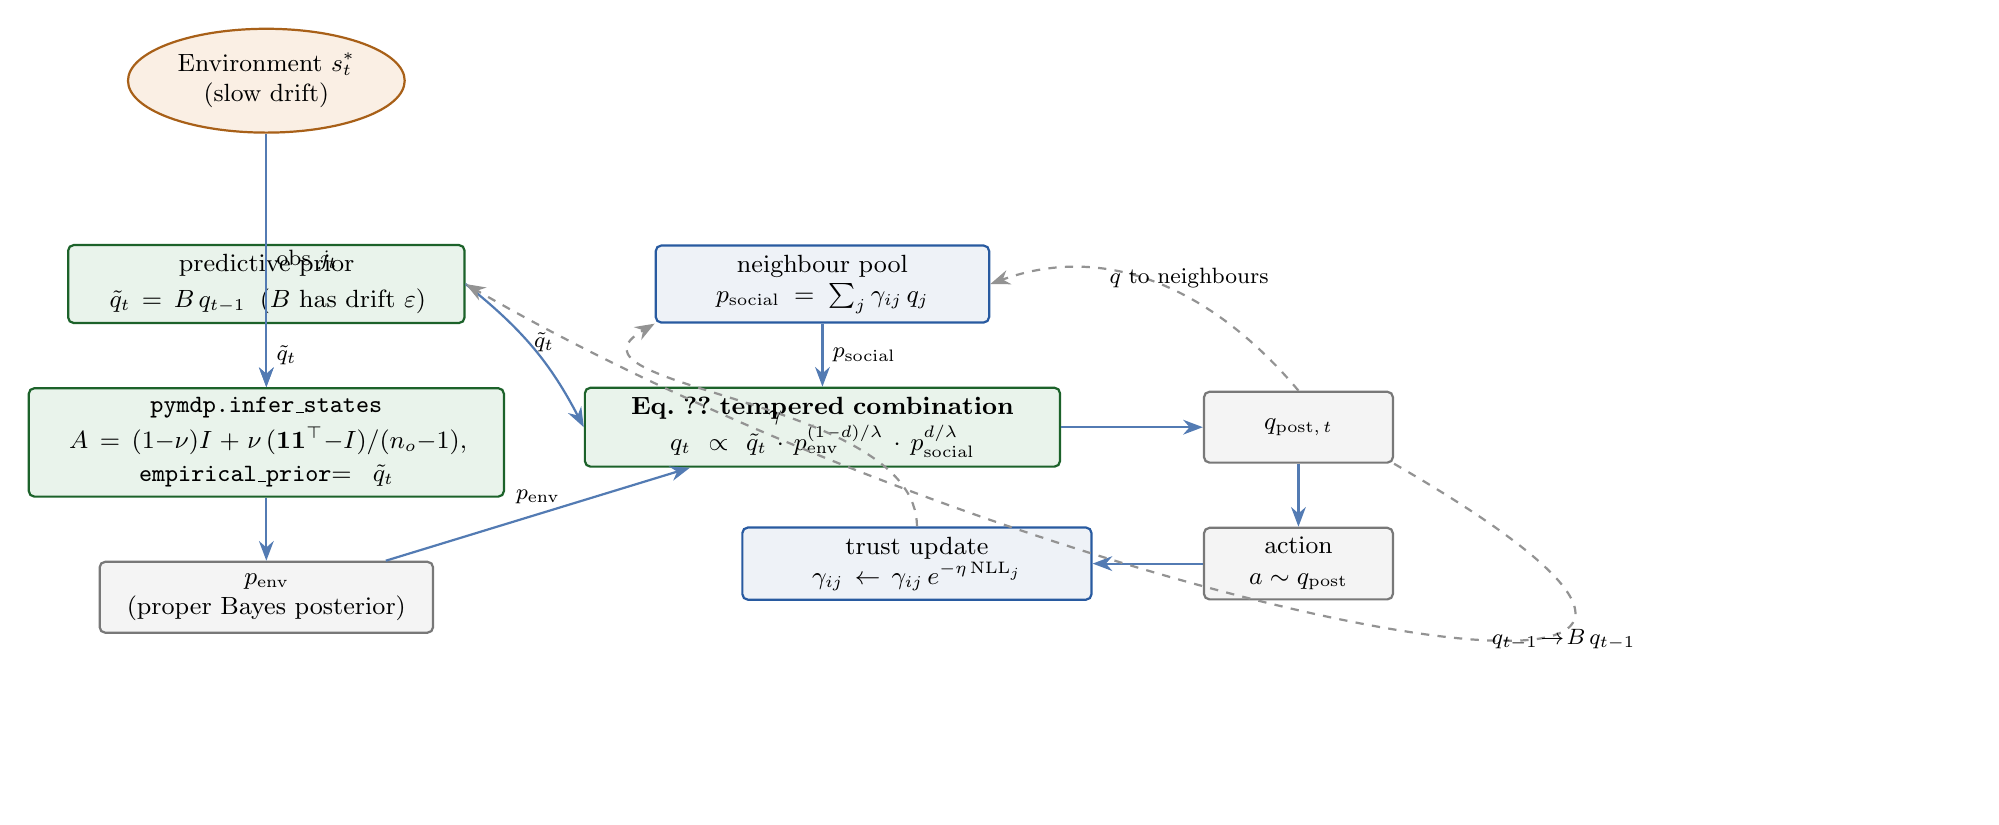
\begin{tikzpicture}[node distance=10mm and 18mm]

% Environment
\node[env] (env) {Environment $s^*_t$\\(slow drift)};

% Drift step (B applied to last posterior)
\node[procfix, below=14mm of env, text width=48mm] (drift) {%
  predictive prior\\[2pt]
  $\tilde q_t = B\,q_{t-1}$\;\;($B$ has drift $\varepsilon$)
};

% pymdp.infer_states with softened A and recursive prior
\node[procfix, below=8mm of drift, text width=58mm] (infer) {%
  \code{pymdp.infer\_states}\\[2pt]
  $A=(1{-}\nu)I + \nu\,(\mathbf{1}\mathbf{1}^\top{-}I)/(n_o{-}1)$,\\[1pt]
  \code{empirical\_prior}$=\tilde q_t$
};
\draw[arr] (env) -- node[right, font=\footnotesize] {obs $j_t$} (infer);
\draw[arr] (drift) -- node[right, font=\footnotesize] {$\tilde q_t$} (infer);

% p_env state
\node[state, below=8mm of infer, text width=40mm] (penv) {$p_{\text{env}}$ \\ (proper Bayes posterior)};
\draw[arr] (infer) -- (penv);

% neighbour pool right of drift
\node[proc, right=24mm of drift, text width=40mm] (npool) {%
  neighbour pool\\$p_{\text{social}} = \sum_j \gamma_{ij}\,q_j$
};

% Eq 13 tempered combination
\node[procfix, below=8mm of npool, text width=58mm] (upd) {%
  \textbf{Eq.~\ref{eq:eq13} tempered combination}\\[2pt]
  $q_t \propto \tilde q_t \cdot p_{\text{env}}^{(1-d)/\lambda} \cdot p_{\text{social}}^{d/\lambda}$
};
\draw[arr] (npool) -- node[right, font=\footnotesize] {$p_{\text{social}}$} (upd);
\draw[arr] (penv) -- node[above, font=\footnotesize] {$p_{\text{env}}$} (upd);
\draw[arr] (drift.east) to[bend left=12] node[above, font=\footnotesize, pos=0.6] {$\tilde q_t$} (upd.west);

% q_post
\node[state, right=18mm of upd] (qpost) {$q_{\text{post},\,t}$};
\draw[arr] (upd) -- (qpost);

% action
\node[state, below=8mm of qpost] (act) {action\\$a \sim q_{\text{post}}$};
\draw[arr] (qpost) -- (act);

% trust update
\node[proc, left=14mm of act, text width=42mm] (trust) {trust update\\$\gamma_{ij}\!\leftarrow\!\gamma_{ij}\,e^{-\eta\,\mathrm{NLL}_j}$};
\draw[arr] (act) -- (trust);

% TEMPORAL LOOP: q_post -> drift block (B q_{t-1})
\draw[arrloop] (qpost.south east) to[out=-30, in=-30, looseness=1.8]
   node[right, font=\footnotesize, pos=0.4] {$q_{t-1}\!\to\! B\,q_{t-1}$}
   (drift.east);

% q_post -> neighbour pool (other agents)
\draw[arrloop] (qpost.north) to[out=130, in=20]
   node[above, font=\footnotesize, pos=0.4] {$q$ to neighbours}
   (npool.east);

% trust feeds neighbour_pool
\draw[arrloop] (trust.north) to[out=90, in=-150]
   node[left, font=\footnotesize, pos=0.4] {$\gamma$}
   (npool.south west);

\end{tikzpicture}
\caption{Information flow under the proposed fix. Green boxes are the
changed components; the temporal loop now passes through the transition
matrix $B$, where active-inference theory expects it. The social and trust
loops are unchanged.}
\label{fig:proposed}
\end{figure}

% --------------------------------------------------------------------------
\section{Mapping back to the original plan}
\label{sec:mapping}

\paragraph{Verification criteria.} The notebook-level verification criteria
in the prior implementation plan (\code{notebooks/02\_phase\_space.ipynb}
\S0--\S5) are unchanged in shape. They will be re-checked against the
proposed dynamics:

\begin{table}[h]
\centering
\small
\begin{tabular}{@{}l l l@{}}
\toprule
\textbf{Criterion} & \textbf{Holds under v02?} & \textbf{Should hold under fix?} \\
\midrule
\S0 \code{type(pop.agent).\_\_name\_\_ == "Agent"} & \checkmark & \checkmark \\
\S1 mean-payoff varies smoothly & partially (saturates) & \checkmark (bounded $|C|$) \\
\S2 monotone $(\lambda, \text{drift})$ degradation & \emph{fails} ($\lambda$-flat) &
   \checkmark expected: $\lambda$ now controls likelihood weight \\
\S3 4 distributions visibly distinct & \checkmark (in narrow window) & \checkmark cleaner \\
\S4 cascade signature in C-trajectories & \checkmark & \checkmark cleaner \\
\S5 dissent front spreading visibly & \checkmark (after viz fix) & \checkmark \\
\bottomrule
\end{tabular}
\end{table}

\paragraph{Experimental plan.} The brief's E1--E4 sequence
(\code{notes/theory\_brief.md}, \S Experimental plan) is unaffected at the
\emph{plan} level. The deadlines (E1: 2026-05-14, E2: 2026-05-15--17, E3:
2026-05-18--21, E4: 2026-05-24--27) require the new architecture be in place
within $\sim$5 days. The four-piece change is small (one config field, one
agent.py function, two lines in population.py setup, two lines in
\code{\_observe\_jit}); estimated implementation time is one focused
session.

\paragraph{What's still out of scope.} The Leibo and Tan Zhi-Xuan critiques
(action-channel observation, theory-of-mind over neighbours) are not
addressed by this fix. They are deferred to a follow-up slice if results
support the paper's claim. The dissociation experiment vs.\ rule-induction
(E4) does \emph{not} require those critiques to be addressed --- it requires
the asymmetric $\lambda$-cost mechanism to do meaningful work, which the
proposed fix is what enables.

% --------------------------------------------------------------------------
\section{Decision summary}
\label{sec:decision}

\begin{enumerate}[topsep=2pt,itemsep=2pt]
\item Adopt the four-piece change in Table~\ref{tab:fix}.
\item Remove \code{memory\_persistence} from \code{ModelConfig} (it was the
  $\beta$ patch; no longer needed).
\item Add \code{obs\_noise} ($\nu$, default $0.05$) and \code{state\_drift}
  ($\varepsilon$, default $0.02$) to \code{ModelConfig}.
\item Replace \code{src/agent.py::update\_belief} with the tempered
  product-of-likelihoods form.
\item Re-execute \code{notebooks/02\_phase\_space.ipynb} and re-check
  verification criteria \S1--\S5.
\item If \S2 still shows $\lambda$-flat behaviour, sweep $\lambda$ over a
  wider range (e.g.\ $\{0.1, 0.3, 1.0, 3.0, 10.0\}$ instead of $\{0.1, 0.5,
  1.5, 5.0\}$); the change in dynamics may be located outside the previous
  window.
\end{enumerate}

\end{document}
